\section{Perturbed bows}
\label{sec:perturbed-bows}

\begin{figure*}
  \centering
  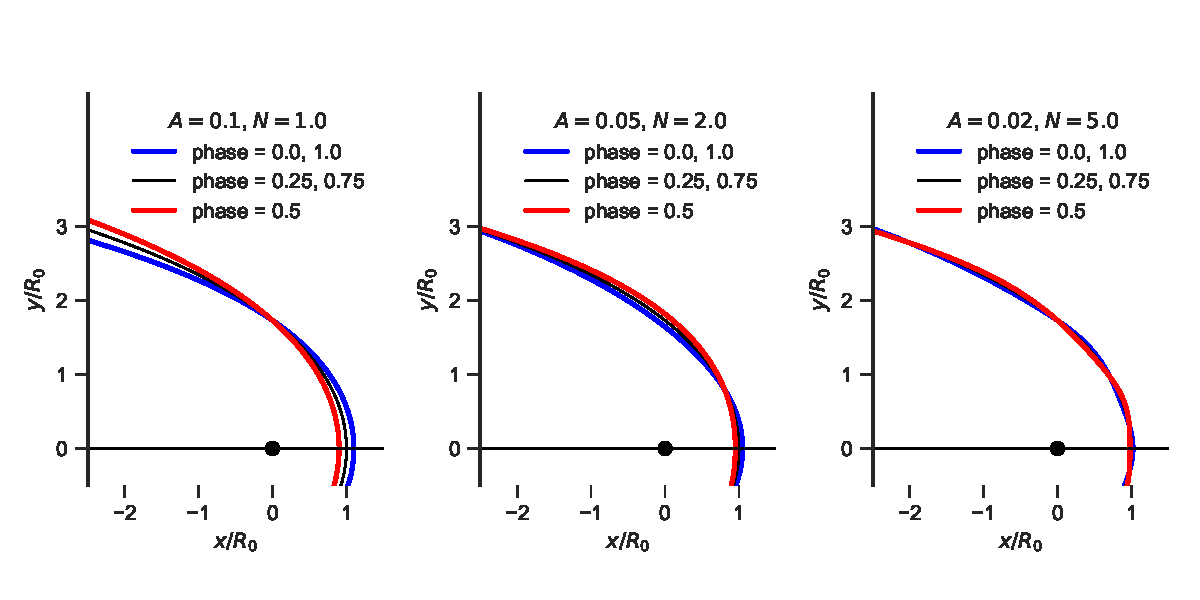
\includegraphics[width=\linewidth]{figs/compare_xyprime_wave-wilkinoid}
  \caption{Small-amplitude standing wave perturbations to bow shapes.}
  \label{fig:perturb-shapes}
\end{figure*}

\begin{figure*}
  \centering
  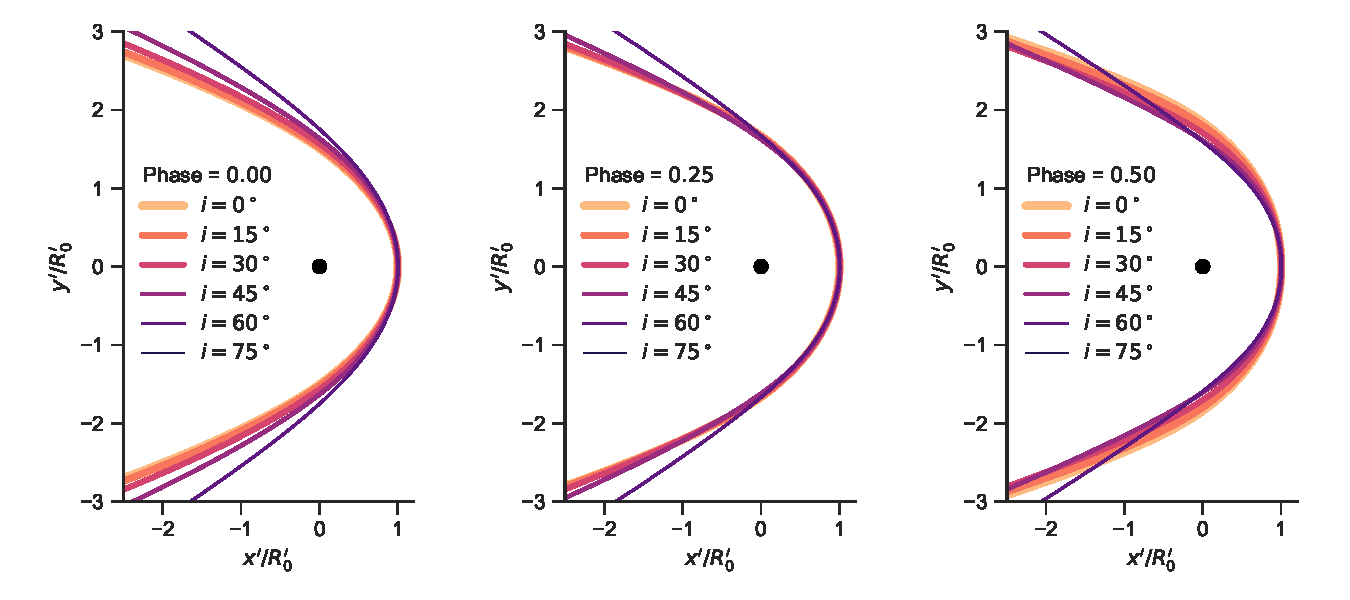
\includegraphics[width=\linewidth]
  {figs/wave_xyprime-A005-N20-ancantoid-xi080-beta000500}
  \caption{Plane-of-sky projections of perturbed bow shapes}
  \label{fig:perturb-xy-prime}
\end{figure*}

The bow shock models that we have considered so far have been
steady-state: although material is moving throughout the bow, the
pattern of its structure does not vary with time.  In this section, we
consider small, time-varying perturbations to such a steady-state
structure.  These may be due to periodic variations in the
momentum-loss rate of one of the winds, or due to dynamical
instabilities in the shocked shell.

For simplicity, we consider standing waves with an amplitude that
multiplies the bow shock radius \(R\) and a pattern that is periodic
in the axial angle \(\theta\): \(R(\theta) \to (1 + \Delta) R(\theta)\), where
\begin{equation}
  \label{eq:standing-wave}
  \Delta = A \cos(N \theta) \cos(2\pi \varphi)
\end{equation}

\begin{figure}
  \centering
  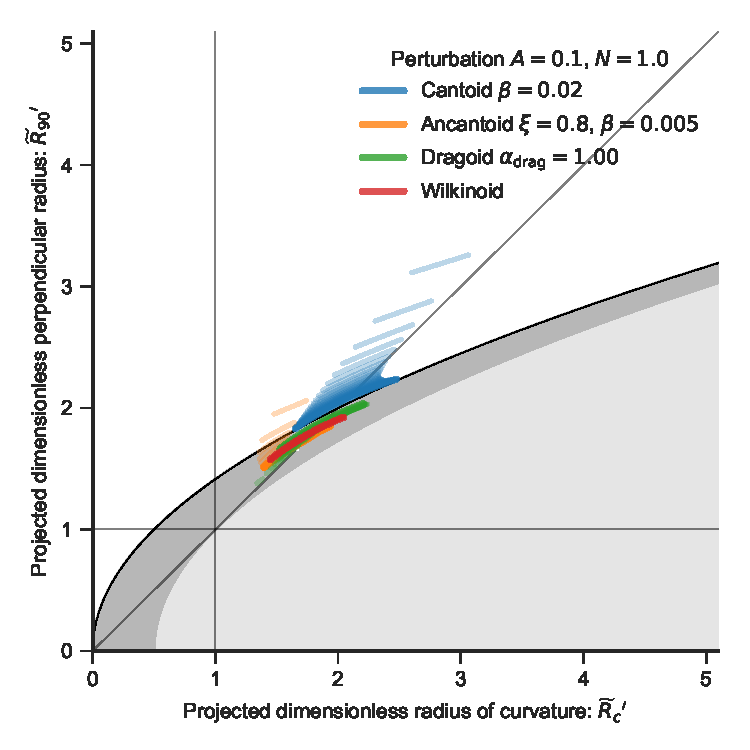
\includegraphics[width=\linewidth]
  {figs/wave-R90-vs-Rc-A010-N10}
  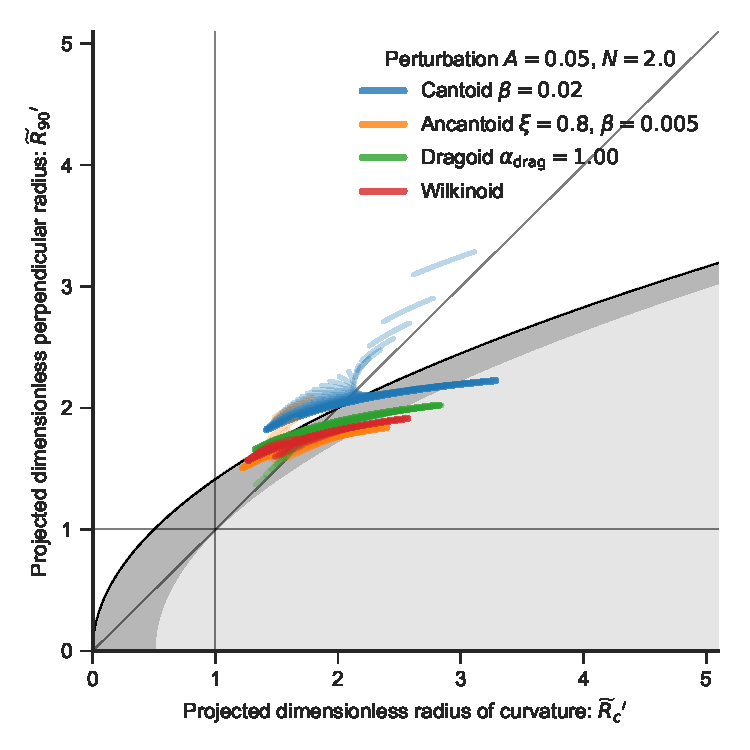
\includegraphics[width=\linewidth]
  {figs/wave-R90-vs-Rc-A005-N20}
  \caption{Diagnostic diagram for perturbed shapes}
  \label{fig:perturb-Rc-R90}
\end{figure}


%%% Local Variables:
%%% mode: latex
%%% TeX-master: "quadrics-bowshock"
%%% End:
